% ============================================================
%  The Particle Model — Lesson Booklet (one section per lesson: A Reading · B Theory · C Practice · D Above level)
%  Year 7 (Year 8 extension)  |  Victorian Curriculum F–10 Version 2.0
%  Compile with: xelatex three times, then python3 fill.py Particle_Model_Lesson_Booklet_Yr7
% ============================================================
\documentclass[11pt,a5paper,twoside]{article}
\newcommand{\wrcoverfile}{../../../covers/ecosystems.jpg}\newcommand{\unitname}{Biodiversity and Ecosystems}\newcommand{\unitcaps}{BIODIVERSITY AND ECOSYSTEMS}

% ── Fonts (compile with LuaLaTeX) ────────────────────────────────────────────
\usepackage{fontspec}
% Bundled fonts (in ./fonts/) so the document compiles anywhere with XeLaTeX/LuaLaTeX
\setmainfont{Lato}[                   % body — humanist sans (stands in for deck's Inter)
  Path=../fonts/, Extension=.ttf, Ligatures=TeX,
  UprightFont=Lato-Regular, ItalicFont=Lato-Italic,
  BoldFont=Lato-Bold, BoldItalicFont=Lato-BoldItalic ]
\newfontfamily\headingfont{Poppins}[  % display/headings — matches the slide decks
  Path=../fonts/, Extension=.ttf, Ligatures=TeX,
  UprightFont=Poppins-Regular, ItalicFont=Poppins-Italic,
  BoldFont=Poppins-Bold, BoldItalicFont=Poppins-BoldItalic ]
\setlength{\headheight}{22pt}

\usepackage[protrusion=true,expansion=false]{microtype}
\usepackage[a5paper, inner=17mm, outer=13mm, top=19mm, bottom=17mm, headheight=14pt, headsep=4mm, footskip=8mm]{geometry}
\usepackage{xcolor}
\usepackage{tikz}
\usetikzlibrary{arrows.meta, shapes.geometric, calc, positioning, decorations.pathreplacing}
\usepackage{tcolorbox}
\tcbuselibrary{skins, breakable, raster}
\usepackage{fancyhdr}
\usepackage{titlesec}
\usepackage{enumitem}
\usepackage{booktabs}
\usepackage{tabularx}
\usepackage{array}
\usepackage{colortbl}
\usepackage{multicol}
\usepackage{amsmath}
\usepackage{needspace}
% TikZ diagram macros are embedded below (just before \begin{document}) for easy editing.
\usepackage{longtable}
\usepackage{graphicx}
\usepackage{pifont}
\usepackage{lastpage}
\usepackage{calc}
\usepackage{mdframed}
\usepackage{setspace}
\usepackage{ragged2e}
% PDF bookmarks: one per lesson (made in \sectiondiv) plus the cover and
% contents, and links from the contents table to each lesson.
% implicit=false: hyperref adds no anchors of its own (an anchor on each
% list item nudged lists down 1.5 mm, which would undo the page fill).
% hidelinks keeps the links invisible, so the printed pages are unchanged.
\usepackage[implicit=false, hidelinks,
  pdftitle={Biodiversity and Ecosystems — Lesson Booklet},
  pdfsubject={Years 7–8 Science, Victorian Curriculum F–10 v2.0}]{hyperref}
\usepackage{bookmark} % writes the outline itself, which implicit=false switches off in hyperref
% hyperref 7.01 with implicit=false leaves \Hy@PageAnchorSlide undefined, which
% throws at \end{document} and stops fill.py (it builds with -halt-on-error).
\makeatletter\providecommand\Hy@PageAnchorSlide{}\makeatother

% ── Colour Palette ───────────────────────────────────────────────────────────
% Remapped to the slide-deck palette (names kept so body + diagrams cascade)
\definecolor{NavyBlue}   {HTML}{16305C}
\definecolor{MidBlue}    {HTML}{2E6FE0}
\definecolor{LightBlue}  {HTML}{E8F1FF}
\definecolor{TealGreen}  {HTML}{0F6E63}
\definecolor{LightGreen} {HTML}{E0F7F3}
\definecolor{GoldDark}   {HTML}{C77F12}
\definecolor{GoldLight}  {HTML}{FFF3DC}
\definecolor{PurpleDark} {HTML}{5B3FC0}
\definecolor{PurpleLight}{HTML}{EFE9FF}
\definecolor{OrangeDark} {HTML}{C9483D}
\definecolor{OrangeLight}{HTML}{FFE9E6}
\definecolor{MidGrey}    {HTML}{AEBED4}
\definecolor{LightGrey}  {HTML}{F2F5FA}
\definecolor{DarkGrey}   {HTML}{3A4759}
\definecolor{TableHead}  {HTML}{16305C}
\definecolor{RowAlt}     {HTML}{EEF4FF}
% Bright accent tints (deck) for bars, rules and chips
\definecolor{Blue}   {HTML}{2E6FE0}
\definecolor{Teal}   {HTML}{18A999}
\definecolor{Amber}  {HTML}{F5A623}
\definecolor{Coral}  {HTML}{FF6B5E}
\definecolor{Violet} {HTML}{7C5CE0}
\definecolor{Sky}    {HTML}{4DA3FF}
\definecolor{Ink}    {HTML}{16223A}
\definecolor{Line}   {HTML}{DDE5F0}
\definecolor{Paper}  {HTML}{FBFCFE}

% ── Page Style ───────────────────────────────────────────────────────────────
\pagestyle{fancy}
\fancyhf{}
\renewcommand{\headrulewidth}{0.4pt}
\renewcommand{\headrule}{\hbox to\headwidth{\color{NavyBlue}\leaders\hrule height \headrulewidth\hfill}}
\fancyhead[L]{\headingfont\small\color{NavyBlue}The Particle Model}
\fancyhead[R]{\headingfont\small\color{DarkGrey}Year 7 \textbar{} Victorian Curriculum F--10 v2.0}
\fancyfoot[C]{\headingfont\small\color{DarkGrey}\thepage\ \textbar{} \pageref{LastPage}}
\fancypagestyle{plain}{%
  \fancyhf{}
  \fancyfoot[C]{\headingfont\small\color{DarkGrey}\thepage\ \textbar{} \pageref{LastPage}}
  \renewcommand{\headrulewidth}{0pt}
}

% ── Section Formatting ───────────────────────────────────────────────────────
\titleformat{\section}
  {\headingfont\color{NavyBlue}\Large\bfseries}
  {}{0em}{}
  [{\color{Teal}\rule[0.6ex]{2.2em}{3pt}}{\color{Line}\rule[0.6ex]{\dimexpr\linewidth-2.2em\relax}{1pt}}]
\titlespacing{\section}{0pt}{18pt}{8pt}

\titleformat{\subsection}
  {\headingfont\color{MidBlue}\large\bfseries}
  {\thesubsection}{0.6em}{}
\titlespacing{\subsection}{0pt}{12pt}{4pt}

\titleformat{\subsubsection}
  {\headingfont\color{NavyBlue}\normalsize\bfseries}
  {}{0em}{}
\titlespacing{\subsubsection}{0pt}{8pt}{2pt}

% Deck-style eyebrow / kicker (optional use)
\newcommand{\kicker}[2][Teal]{%
  {\headingfont\bfseries\footnotesize\color{#1}%
   \textcolor{#1}{\rule[0.18ex]{1.6em}{2.2pt}}\hspace{0.5em}\MakeUppercase{#2}\par}%
  \vspace{2pt}}

% ── Custom tcolorbox Environments ────────────────────────────────────────────

% Section divider banner
\newtcolorbox{sectionbanner}[2]{
  enhanced, breakable=false,
  colback=NavyBlue, colframe=NavyBlue,
  fontupper=\color{white}\bfseries\large,
  left=4mm, right=4mm, top=3mm, bottom=3mm,
  title={\color{white}\Huge\bfseries #1},
  attach boxed title to top left={yshift=-2mm, xshift=4mm},
  boxed title style={colback=NavyBlue, colframe=NavyBlue},
  after upper={\par\smallskip\normalfont\normalsize\color{white!80!NavyBlue}\textit{#2}}
}

% Key info box (blue)
\newtcolorbox{infobox}[1]{
  breakable, arc=2.5mm, boxrule=0.5pt,
  colback=LightBlue, colframe=Blue!40,
  fonttitle=\headingfont\bfseries, coltitle=MidBlue,
  title={#1},
  left=4mm, right=3.5mm, top=2.5mm, bottom=2.5mm
}

% Scaffold box (yellow)
\newtcolorbox{scaffold}[1]{
  breakable, arc=2.5mm, boxrule=0.5pt,
  colback=GoldLight, colframe=Amber!40,
  fonttitle=\headingfont\bfseries, coltitle=GoldDark,
  title={#1},
  left=4mm, right=3.5mm, top=2.5mm, bottom=2.5mm
}

% Worked example box
\newtcolorbox{workedexbox}[1]{
  breakable, arc=2.5mm, boxrule=0.5pt,
  colback=white, colframe=Amber!50,
  fonttitle=\headingfont\bfseries, coltitle=GoldDark,
  title={#1},
  left=4mm, right=3.5mm, top=2.5mm, bottom=2.5mm
}
% Worked examples: \begin{workedex}{title} -> "Worked Example N.M --- title",
% auto-numbered per section and labelled we:N.M. Never type the number.
\newcounter{wenum}[section]
\renewcommand{\thewenum}{\thesection.\arabic{wenum}}
\newenvironment{workedex}[1]
  {\refstepcounter{wenum}\label{we:\thewenum}\begin{workedexbox}{Worked Example \thewenum\ --- #1}}
  {\end{workedexbox}}

% We do: straight after each worked example, a near-identical question the
% class works through together, with its own writing space. Numbered to
% match the worked example above it and labelled wd:N.M.
%   \begin{wedo}{title} question ... \answerbox{h} \end{wedo}
\newtcolorbox{wedobox}[1]{
  enhanced, breakable=false, arc=2.5mm, boxrule=0.5pt,
  colback=white, colframe=TealGreen!55,
  fonttitle=\headingfont\bfseries, coltitle=TealGreen!75!black,
  title={#1},
  left=4mm, right=3.5mm, top=2.5mm, bottom=2.5mm
}
\newenvironment{wedo}[1]
  {\par\needspace{9\baselineskip}\begin{wedobox}{We do \thewenum\ --- #1}\label{wd:\thewenum}\ignorespaces}
  {\end{wedobox}}

% Year 7 box (blue)
\newtcolorbox{yr7box}{
  breakable, arc=2.5mm, boxrule=0.5pt,
  colback=LightBlue, colframe=Blue!40,
  left=4mm, right=3.5mm, top=2.5mm, bottom=2.5mm
}

% Year 8 extension box (violet)
\newtcolorbox{yr8box}{
  breakable, arc=2.5mm, boxrule=0.5pt,
  colback=PurpleLight, colframe=Violet!40,
  left=4mm, right=3.5mm, top=2.5mm, bottom=2.5mm
}

% Answer lines box
\newcommand{\answerbox}[1]{%
  \begin{tcolorbox}[
    enhanced, breakable, arc=2mm,
    colback=Paper, colframe=Line,
    left=2mm, right=2mm, top=1mm, bottom=1mm,
    boxrule=1pt,
    height=#1
  ]
  \end{tcolorbox}%
}

% Experiment header
\newtcolorbox{expheader}[3]{
  breakable=false, arc=2.5mm,
  colback=RowAlt, colframe=Amber!50, boxrule=0.5pt,
  fonttitle=\headingfont\bfseries\large, coltitle=NavyBlue,
  title={Experiment #1: #2},
  left=4mm, right=3.5mm, top=2.5mm, bottom=2.5mm,
  after upper={\par\smallskip
    {\headingfont\bfseries\color{GoldDark}Aim:}\ \textit{#3}},
}

% Reading comprehension passage box (green)
\newtcolorbox{readingbox}[1]{
  breakable, arc=2.5mm, boxrule=0.5pt,
  colback=white, colframe=Teal!50,
  fonttitle=\headingfont\bfseries, coltitle=TealGreen,
  title={#1},
  left=4mm, right=3.5mm, top=2.5mm, bottom=2.5mm,
  fontupper=\normalsize
}

% Skill-builder box (for beginner scaffolding)
\newtcolorbox{skillbox}[1]{
  breakable, arc=2.5mm, boxrule=0.5pt,
  colback=RowAlt, colframe=Blue!40,
  fonttitle=\headingfont\bfseries, coltitle=MidBlue,
  title={#1},
  left=4mm, right=3.5mm, top=2.5mm, bottom=2.5mm
}

% ── Custom Commands ───────────────────────────────────────────────────────────

% Question: \question{marks}{text}  (marks can be empty)
% Numbered automatically as Q<section>.<n>, reset every section.
% Do NOT write numbers by hand.
\newcounter{qnum}[section]
\renewcommand{\theqnum}{\thesection.\arabic{qnum}}
\newcommand{\question}[2]{%
  \refstepcounter{qnum}%
  \needspace{3\baselineskip}%
  \medskip
  \noindent\label{q:\theqnum}\textbf{Q\theqnum}\ifx&#1&\else\ \textcolor{DarkGrey}{(#1 mark\ifnum#1=1\else s\fi)}\fi\quad #2%
  \medskip
}

% Inline marks note
\newcommand{\markscount}[1]{\hfill\textcolor{DarkGrey}{\textit{(#1 mark\ifnum#1=1\else s\fi)}}}

% ── Practice set counter and question macros ─────────────────────────────────
\newcounter{pqnum}
\newcommand{\practiceset}[1]{%
  \needspace{6\baselineskip}
  \setcounter{pqnum}{0}%
  \vspace{6pt}
  {\headingfont\bfseries\large\color{GoldDark} Practice Set --- #1}\\[-2pt]
  {\color{Amber}\rule{\linewidth}{1pt}}\\[2pt]
}
% \pq{question text}{working box height}
\newcommand{\pq}[2]{%
  \stepcounter{pqnum}%
  \needspace{4\baselineskip}
  \vspace{5pt}
  \noindent\textbf{\thepqnum.}\quad #1\par
  \vspace{2pt}
  \answerbox{#2}
}
% Two short questions side by side, each with its own box
\newcommand{\pqpair}[4]{%
  \needspace{4\baselineskip}
  \vspace{5pt}
  \noindent
  \begin{minipage}[t]{0.48\linewidth}
    \stepcounter{pqnum}\textbf{\thepqnum.}\quad #1\par\vspace{2pt}
    \begin{tcolorbox}[enhanced,arc=2mm,colback=Paper,colframe=Line,left=2mm,right=2mm,
      top=1mm,bottom=1mm,boxrule=1pt,height=#2]\end{tcolorbox}
  \end{minipage}\hfill
  \begin{minipage}[t]{0.48\linewidth}
    \stepcounter{pqnum}\textbf{\thepqnum.}\quad #3\par\vspace{2pt}
    \begin{tcolorbox}[enhanced,arc=2mm,colback=Paper,colframe=Line,left=2mm,right=2mm,
      top=1mm,bottom=1mm,boxrule=1pt,height=#4]\end{tcolorbox}
  \end{minipage}
}

% ── Comprehension question macro (compact, lined) ────────────────────────────
\newcounter{rcnum}
\newcommand{\rcreset}{\setcounter{rcnum}{0}}
\newcommand{\rcq}[2]{%
  \stepcounter{rcnum}%
  \needspace{3\baselineskip}
  \vspace{4pt}
  \noindent\textbf{C\thercnum.}\quad #1\par
  \vspace{2pt}
  \linedbox{#2}
}

% Section divider (big numbered banner): \sectiondiv{title}{summary}
%
% This IS the section: it steps the real section counter, so subsections,
% tasks, questions and figures inside it are numbered N.M automatically.
% Put \label{sec:N} straight after it. Never hand-type a section number.
\newcommand{\sectiondiv}[2]{%
  \needspace{5\baselineskip}%
  \refstepcounter{section}%
  % PDF bookmark for the lesson; its anchor, lesson.N.1, is what the contents table links to
  \pdfbookmark[1]{Lesson \thesection{} — #1}{lesson.\thesection}%
  \begin{tcolorbox}[
    enhanced, breakable=false, arc=3.5mm,
    colback=NavyBlue, colframe=NavyBlue, boxrule=0pt,
    sidebyside, sidebyside align=center,
    lefthand width=2.4cm,
    left=2mm, right=4mm, top=4mm, bottom=4mm
  ]
    \begin{center}
      {\headingfont\bfseries\color{white!35!NavyBlue}\fontsize{50}{50}\selectfont \thesection}
    \end{center}
    \tcblower
    {\headingfont\bfseries\color{white}\LARGE #1}\\[3pt]
    {\itshape\color{white!75!NavyBlue}\small #2}
  \end{tcolorbox}%
}

% Tasks: \task, \task[a] (part a of a NEW task), \taskpart{b} (next part
% of the same task), \exttask (Year 8 "Extension" — same counter).
% Numbered Task <section>.<n>, reset every section. Do NOT type numbers.
% Every task, question and figure also gets an automatic label
% (task:1.7b, q:2.4, fig:1.2, fig:E2.1) so page refs come from the .aux.
\newcounter{tasknum}[section]
\renewcommand{\thetasknum}{\thesection.\arabic{tasknum}}
\NewDocumentCommand{\task}{o}{\refstepcounter{tasknum}\label{task:\thetasknum\IfValueT{#1}{#1}}\textbf{Task \thetasknum\IfValueT{#1}{#1}}}
\newcommand{\taskpart}[1]{\label{task:\thetasknum#1}\textbf{Task \thetasknum#1}}
\newcommand{\exttask}{\refstepcounter{tasknum}\label{task:\thetasknum}\textbf{Extension \thetasknum}}

% Figure captions: \figcap[fig:label]{caption} -> "Figure N.M --- caption"
% \expfigcap{caption} -> "Figure EN.M" (experiment pages). Both auto-numbered.
\newcounter{fignum}[section]
\renewcommand{\thefignum}{\thesection.\arabic{fignum}}
\newcounter{expfignum}[section]
\renewcommand{\theexpfignum}{E\thesection.\arabic{expfignum}}
\newcommand{\figcap}[2][]{%
  \begin{center}
    \refstepcounter{fignum}\label{fig:\thefignum}\if\relax\detokenize{#1}\relax\else\label{#1}\fi
    \small\itshape\color{DarkGrey} Figure \thefignum\ --- #2
  \end{center}%
}
\newcommand{\expfigcap}[1]{%
  \begin{center}
    \refstepcounter{expfignum}\label{fig:\theexpfignum}%
    \small\itshape\color{DarkGrey} Figure \theexpfignum\ --- #1
  \end{center}%
}

% Diagram include
\newcommand{\diagramfig}[3]{%  {filename}{width fraction}{caption}
  \begin{center}
    \includegraphics[width=#2\linewidth]{#1}\\[4pt]
    \small\itshape\color{DarkGrey} #3
  \end{center}%
}

% Table column types
\newcolumntype{L}[1]{>{\RaggedRight\arraybackslash}p{#1}}
\newcolumntype{C}[1]{>{\Centering\arraybackslash}p{#1}}

% Table header colour
\newcommand{\thead}[1]{\cellcolor{TableHead}\color{white}\bfseries #1}
\newcommand{\talt}{\rowcolor{RowAlt}}
\newcommand{\tmid}{\rowcolor{MidGrey}}

% Inline year tags
\newcommand{\tagyr}[1]{%
  \tikz[baseline=-0.5ex]\node[
    rounded corners=2pt,
    fill=#1!20, draw=#1, text=#1,
    inner xsep=4pt, inner ysep=1pt,
    font=\scriptsize\bfseries
  ]{Yr #1 only};}

% Draw answer lines
\newcommand{\anslines}[1]{%
  \vspace{2pt}%
  \foreach \n in {1,...,#1}{%
    \par\noindent\rule{\linewidth}{0.3pt}\vspace{3pt}%
  }%
}

% ── Document ─────────────────────────────────────────────────────────────────
% ── Optional-lesson note, shown under the lesson banner ──────────────────────
\newcommand{\optionalnote}[1]{%
  % the title is a bold lead-in on the first line rather than a title bar,
  % which keeps Lesson 11's reading on the lesson's first page
  \begin{tcolorbox}[enhanced, breakable=false, arc=2.5mm, boxrule=0.5pt,
    colback=PurpleLight, colframe=Violet!50,
    left=4mm, right=3.5mm, top=2mm, bottom=2mm]
  {\headingfont\bfseries\color{PurpleDark}Optional lesson \textbullet{} Year 8 extension.}\enspace #1
  \end{tcolorbox}\vspace{2pt}}


% ══════════════════════════════════════════════════════════════════════════════
%  LESSON STRUCTURE (lesson booklet, Oct 2026)
%  Every lesson runs in the same four parts, in this order:
%    \lessonpart{A}{Reading and comprehension}{Teal}   \label{read:N}
%    \lessonpart{B}{Theory and examples}{Blue}         \label{theory:N}
%    \lessonpart{C}{Practice}{Amber}                    \label{prac:N}
%    \lessonpart{D}{Above level}{Violet}                \label{ext:N}
%  Above-level / higher-order questions live ONLY in Part D, at the end.
% ══════════════════════════════════════════════════════════════════════════════
\newcommand{\lessonpart}[3]{%
  \par\if#1A\needspace{10\baselineskip}\vspace{10pt}\else
    \if#1C\notesfill\fi\clearpage\fi
  \begin{tcolorbox}[enhanced, breakable=false, arc=2mm, boxrule=0pt,
    colback=#3!14, borderline west={4pt}{0pt}{#3},
    left=4mm, right=3mm, top=1.6mm, bottom=1.6mm]
  {\headingfont\bfseries\color{#3!60!black}\large Part #1 \textbullet{} #2}
  \end{tcolorbox}\vspace{2pt}}

% Key vocabulary at the start of each lesson: students copy each definition
% from the vocabulary slide in the lesson's starter. First row = red scaffold.
\newcommand{\vocabhead}{%
  \par\vspace{6pt}%
  \begin{tcolorbox}[enhanced, breakable=false, arc=2mm, boxrule=0pt,
    colback=NavyBlue!10, borderline west={4pt}{0pt}{NavyBlue},
    left=4mm, right=3mm, top=1.6mm, bottom=1.6mm]
  {\headingfont\bfseries\color{NavyBlue}\large Key vocabulary}
  \end{tcolorbox}\vspace{2pt}%
  \noindent Copy the definition of each word from the slide. The first one has been done for you.\par}

% Curriculum codes under a lesson banner
\newcommand{\lessoncodes}[1]{%
  {\small\headingfont\color{DarkGrey}Victorian Curriculum 2.0:\ \textbf{#1}}\par\vspace{4pt}}

% Two short tasks side by side, each with its own working box
% \taskpair{text}{box height}{text}{box height}
% The two boxes line up: the shorter question is padded by the difference in
% text height (measured in a scratch box, task counter restored, no label).
\newsavebox\tpbox
\newlength\tpA \newlength\tpB
\newcount\tpsaved
\newcommand\tpmeasure[2]{%
  \tpsaved=\value{tasknum}%
  \sbox\tpbox{\vbox{\hsize=0.485\linewidth \linewidth=\hsize \parskip=0pt
    \renewcommand\label[1]{}\task #1\par}}%
  \setlength{#2}{\dimexpr\ht\tpbox+\dp\tpbox\relax}%
  \setcounter{tasknum}{\tpsaved}}
\newcommand{\taskpair}[4]{%
  \par\needspace{9\baselineskip}\vspace{4pt}%
  \tpmeasure{#1}{\tpA}\tpmeasure{#3}{\tpB}%
  \noindent
  \edef\abgrp{\number\numexpr\value{abox}+1\relax}%
  \begin{minipage}[t]{0.485\linewidth}
    \task #1\par\ifdim\tpB>\tpA\vspace{\dimexpr\tpB-\tpA\relax}\fi\vspace{2pt}\answerbox{#2}
  \end{minipage}\hfill
  \begin{minipage}[t]{0.485\linewidth}
    \task #3\par\ifdim\tpA>\tpB\vspace{\dimexpr\tpA-\tpB\relax}\fi\vspace{2pt}\answerbox{#4}
  \end{minipage}\par\gdef\abgrp{0}\vspace{4pt}}
% Two parts of one question side by side, with their answer boxes level:
% \ptpair{a}{part (a) text}{box height}{b}{part (b) text}{box height}.
% The shorter part's text gets space below it to match the longer one.
\newcommand\ptmeasure[3]{%
  \sbox\tpbox{\vbox{\hsize=0.485\linewidth \linewidth=\hsize \parskip=0pt \pt{#1}#2\par}}%
  \setlength{#3}{\dimexpr\ht\tpbox+\dp\tpbox\relax}}
\newcommand{\ptpair}[6]{%
  \ptmeasure{#1}{#2}{\tpA}\ptmeasure{#4}{#5}{\tpB}%
  \par\noindent
  \edef\abgrp{\number\numexpr\value{abox}+1\relax}%
  \begin{minipage}[t]{0.485\linewidth}
    \pt{#1}#2\par\ifdim\tpB>\tpA\vspace{\dimexpr\tpB-\tpA\relax}\fi\answerbox{#3}
  \end{minipage}\hfill
  \begin{minipage}[t]{0.485\linewidth}
    \pt{#4}#5\par\ifdim\tpA>\tpB\vspace{\dimexpr\tpA-\tpB\relax}\fi\answerbox{#6}
  \end{minipage}\par\gdef\abgrp{0}}

% Answer boxes never split across a page (a half box on its own page is useless)
% ── Page filling ────────────────────────────────────────────────────────────
% Every writing box gets an id. Its page is logged to \jobname.abp; fill.py
% measures the empty space left at the foot of each page and shares it out
% among that page's boxes via \jobname.abx (\abset{id}{extra}). Side-by-side
% boxes share a group so they grow together.
\newcounter{abox}
\newwrite\abpos \immediate\openout\abpos=\jobname.abp
\newcommand{\abset}[2]{\expandafter\gdef\csname abx@#1\endcsname{#2}}
\InputIfFileExists{\jobname.abx}{}{}
\def\abgrp{0}
\newcommand{\abnext}{\stepcounter{abox}%
  \edef\abcur{\ifcsname abx@\theabox\endcsname\csname abx@\theabox\endcsname\else 0pt\fi}}
\newcommand{\ablog}{\edef\abtmp{\noexpand\write\abpos{\theabox\space\abgrp\space\noexpand\thepage}}\abtmp}
\newcommand{\abh}[1]{\dimexpr#1+\abcur\relax}
\renewcommand{\answerbox}[1]{%
  \abnext
  \begin{tcolorbox}[enhanced, breakable=false, arc=2mm, colback=Paper, colframe=Line,
    left=2mm, right=2mm, top=1mm, bottom=1mm, boxrule=1pt, height=\abh{#1}]
  \end{tcolorbox}\ablog%
}
% \linedbox{height}: an answer box ruled in dotted thirds. Lines are \thirdrow/3 apart and run dotted, dotted,
% solid (the baseline), repeating, and end on one dotted line. The number of
% rows is worked out from the box's final height, so the ruling still fills the
% box after fill.py has grown it; the rows are centred in the box.
\newlength\thirdrow \setlength\thirdrow{9mm}
\tikzset{thirdsolid/.style={draw=DarkGrey!70, line width=0.5pt},
         thirddot/.style={draw=DarkGrey!70, line width=0.6pt, dash pattern=on 0.9pt off 1.6pt}}
\newlength\lbH \newlength\lbO \newcount\lbN
\newcommand{\linedbox}[1]{%
  \abnext
  % interior height = box height less the 1pt frame top and bottom
  \setlength\lbH{\dimexpr\abh{#1}-2pt\relax}%
  % whole rows that fit with at least 3 mm spare top and bottom (at least one)
  \lbN=\numexpr(\dimexpr\lbH-6mm-\thirdrow/2\relax)/\thirdrow\relax
  \ifnum\lbN<1 \lbN=1 \fi
  \setlength\lbO{\dimexpr(\lbH-\lbN\thirdrow)/2\relax}%
  \begin{tcolorbox}[enhanced, breakable=false, arc=2mm, colback=Paper, colframe=Line,
    left=2mm, right=2mm, top=1mm, bottom=1mm, boxrule=1pt, height=\abh{#1},
    underlay={\begin{tcbclipinterior}
      \foreach \i in {1,...,\the\lbN}{
        \draw[thirddot] ([xshift=3mm,yshift=-\lbO-(\i-1)*\thirdrow]interior.north west) -- ([xshift=-3mm,yshift=-\lbO-(\i-1)*\thirdrow]interior.north east);
        \draw[thirddot] ([xshift=3mm,yshift=-\lbO-(\i-1)*\thirdrow-\thirdrow/3]interior.north west) -- ([xshift=-3mm,yshift=-\lbO-(\i-1)*\thirdrow-\thirdrow/3]interior.north east);
        \draw[thirdsolid] ([xshift=3mm,yshift=-\lbO-(\i-1)*\thirdrow-2*\thirdrow/3]interior.north west) -- ([xshift=-3mm,yshift=-\lbO-(\i-1)*\thirdrow-2*\thirdrow/3]interior.north east);}
      \draw[thirddot] ([xshift=3mm,yshift=-\lbO-\lbN\thirdrow]interior.north west) -- ([xshift=-3mm,yshift=-\lbO-\lbN\thirdrow]interior.north east);
    \end{tcbclipinterior}}]
  \end{tcolorbox}\ablog%
}
% Every written-response box is ruled the same way (Part A comprehension, We do,
% Part C tasks and Part D extensions, including side-by-side pairs). Space for
% mathematical working uses \workbox{height} instead and stays plain, as do
% \drawbox and the write-in tables.
\let\workbox\answerbox   % plain box: mathematical working (calculations) stays unruled
\let\answerbox\linedbox
% \drawbox{height}{contents}: white box for a diagram or drawing
\newcommand{\drawbox}[2]{%
  \abnext
  \begin{tcolorbox}[colback=white, colframe=MidGrey, boxrule=0.5pt, height=\abh{#1}]#2\end{tcolorbox}\ablog}
% Notes box at the end of Part B: fills whatever is left of the page (if worth it)
\newcommand{\notesfill}{\par
  \ifdim\dimexpr\pagegoal-\pagetotal\relax>3.2cm
    \vspace*{\fill}%
    \begin{tcolorbox}[enhanced, breakable=false, arc=2mm, colback=Paper, colframe=Line,
      left=2mm, right=2mm, top=1mm, bottom=1mm, boxrule=1pt,
      height=\dimexpr\pagegoal-\pagetotal-1.0cm\relax]
      {\small\headingfont\color{DarkGrey}Notes}
    \end{tcolorbox}%
  \fi}



% Centred table: wrap every content table in \begin{ctab} ... \end{ctab}
% (figures already centre themselves inside their \diag... macros)
% ctab also registers write-in tables (S column) for page filling: the extra
% height is per row, logged with the row count.
\newenvironment{ctab}{\par\smallskip\begingroup\centering
  \abnext\let\tbcur\abcur\global\wtrows0 }{\par
  \ifnum\wtrows>0 \edef\abtmp{\noexpand\write\abpos{\theabox\space\abgrp\space\noexpand\thepage\space\the\wtrows}}\abtmp\fi
  \endgroup\smallskip}

% ── Booklet formatting rules (Oct 2026) ─────────────────────────────────────
% 1. No marks are shown anywhere in the booklet.
\renewcommand{\markscount}[1]{}
% 2. A task's heading sits on its own line; its text starts on the next
%    line, left aligned. Parts (a), (b)… each start a new line: use \pt{a}.
\RenewDocumentCommand{\task}{o}{\par\noindent\refstepcounter{tasknum}\label{task:\thetasknum\IfValueT{#1}{#1}}\textbf{Task \thetasknum\IfValueT{#1}{#1}}\par\nobreak\noindent\ignorespaces}
\renewcommand{\taskpart}[1]{\par\noindent\label{task:\thetasknum#1}\textbf{Task \thetasknum#1}\par\nobreak\noindent\ignorespaces}
\renewcommand{\exttask}{\par\noindent\refstepcounter{tasknum}\label{task:\thetasknum}\textbf{Extension \thetasknum}\par\nobreak\noindent\ignorespaces}
\newcommand{\pt}[1]{\par\noindent\textbf{(#1)}\ \ignorespaces}
% Workstation pages (Experiment 1): numbered method steps with a hanging
% indent, and a one-line safety reminder under the materials list.
\newcommand{\wsstep}[1]{\par\noindent\hangindent=1.6em\hangafter=1\makebox[1.6em][l]{\textbf{#1}}\ignorespaces}
\newcommand{\wssafety}[1]{\par\smallskip{\small\textcolor{ScaffoldRed}{\headingfont\bfseries Safety:}\ #1}\par}
% 3. Tables have vertical rules between columns and down both sides
%    (write | between and around the columns, e.g. {|L{3cm}|C{2cm}|}).
%    Keep the normal padding at the outer edges (no @{} there): colortbl paints
%    header colour one \tabcolsep past each edge, so trimming the padding makes
%    the header overhang the grid.
\arrayrulecolor{MidGrey}
\setlength{\arrayrulewidth}{0.6pt}
% 4. Write-in tables: W/Z are left/centred columns that centre text
%    vertically; put the S column first (see below).
\newcolumntype{W}[1]{>{\RaggedRight\arraybackslash}m{#1}}
\newcolumntype{Z}[1]{>{\Centering\arraybackslash}m{#1}}
\def\tbcur{0pt}
\newcount\wtrows
\newcommand{\wh}{\global\advance\wtrows1 \rule[\dimexpr-0.75cm-\tbcur/2\relax]{0pt}{\dimexpr1.5cm+\tbcur\relax}}
% S = zero-width first column that makes every row of a write-in table
% at least 1.5 cm tall with its text vertically centred. Start each data
% row with "&"; start the header row with "\hd &" so it stays slim.
\newif\ifnowh
\newcolumntype{S}{@{}>{}c<{\ifnowh\else\wh\fi\global\nowhfalse}@{\hspace{\tabcolsep}}}
\newcommand{\hd}{\global\nowhtrue}
% 5. The first row of a multi-row write-in table is a worked scaffold in red.
\definecolor{ScaffoldRed}{HTML}{C0392B}
\newcommand{\scaf}[1]{\textcolor{ScaffoldRed}{\itshape #1}}
% 6. Tables are a light grid (rules between rows and columns) on white —
%    row shading is off, because colortbl paints shading over column rules.
\renewcommand{\talt}{}
\renewcommand{\tmid}{}
% ══════════════════════════════════════════════════════════════════════════════
%  DIAGRAM DEFINITIONS — The Particle Model
%  Self-contained TikZ macros, no external image files. Each \diag... macro is
%  called from the body by name.
% ══════════════════════════════════════════════════════════════════════════════
\usetikzlibrary{arrows.meta,calc,positioning,patterns,backgrounds}
\tikzset{
  thin arrow/.style={-{Stealth[length=6pt,width=4pt]}, line width=1.4pt},
}

% ── Lesson 1: the same three jars holding a solid, a liquid and a gas ───────────
% The solid keeps its own shape, the liquid takes the jar's shape with a flat top,
% the gas fills the whole jar. No particles yet: those arrive in Lesson 4.
\newcommand{\jar}[1]{% jar outline with its base at (#1,0)
  \draw[line width=1.2pt, Ink] (#1-1.25,2.9) -- (#1-1.25,0.15) arc (180:270:0.15)
    -- (#1+1.1,0) arc (270:360:0.15) -- (#1+1.25,2.9);}
\newcommand{\diagStates}{%
\begin{center}
\begin{tikzpicture}[font=\small, x=1cm, y=1cm]
  % solid: a block sitting in the corner
  \fill[GoldLight] (-0.95,0.02) rectangle (0.15,1.25);
  \draw[GoldDark, line width=1.1pt] (-0.95,0.02) rectangle (0.15,1.25);
  \jar{0}
  \node[font=\bfseries, text=NavyBlue] at (0,-0.45) {Solid};
  \node[align=center, font=\footnotesize, text=DarkGrey] at (0,-1.05) {keeps its own shape\\and volume};
  % liquid: takes the jar's shape, flat top
  \begin{scope}[xshift=4.2cm]
    \fill[Sky!35] (-1.25,0.15) arc (180:270:0.15) -- (1.1,0) arc (270:360:0.15) -- (1.25,1.1) -- (-1.25,1.1) -- cycle;
    \draw[MidBlue, line width=1.1pt] (-1.25,1.1) -- (1.25,1.1);
    \jar{0}
    \node[font=\bfseries, text=NavyBlue] at (0,-0.45) {Liquid};
    \node[align=center, font=\footnotesize, text=DarkGrey] at (0,-1.05) {takes the jar's shape,\\keeps its volume};
  \end{scope}
  % gas: fills the whole (sealed) jar
  \begin{scope}[xshift=8.4cm]
    \fill[Violet!16] (-1.25,0.15) arc (180:270:0.15) -- (1.1,0) arc (270:360:0.15) -- (1.25,2.9) -- (-1.25,2.9) -- cycle;
    \draw[line width=2.2pt, DarkGrey] (-1.4,2.9) -- (1.4,2.9);
    \jar{0}
    \node[font=\scriptsize, text=DarkGrey, anchor=south] at (0,2.95) {lid};
    \node[font=\bfseries, text=NavyBlue] at (0,-0.45) {Gas};
    \node[align=center, font=\footnotesize, text=DarkGrey] at (0,-1.05) {spreads out to fill\\the whole jar};
  \end{scope}
\end{tikzpicture}
\end{center}}

% ── Lesson 1, Worked Example 1.2 and We do 1.2: the same syringe, before and after
\newcommand{\diagSyringe}[3]{% {start mL}{end mL}{contents: gas|liquid}
\begin{center}\resizebox{\linewidth}{!}{%
\begin{tikzpicture}[font=\scriptsize, x=0.11cm, y=1cm]
  \foreach \row/\vol/\lab in {0/#1/before, -1.15/#2/after}{
    \begin{scope}[yshift=\row cm]
      \ifx#3g\fill[Violet!16] (0,0) rectangle (\vol,0.7);\else\fill[Sky!35] (0,0) rectangle (\vol,0.7);\fi
      \draw[line width=1pt, Ink] (0,0) rectangle (60,0.7);
      \draw[line width=1pt, Ink] (0,0.25) -- (-4,0.25) (0,0.45) -- (-4,0.45);
      \fill[Ink] (-5.5,0.15) rectangle (-4,0.55);
      \foreach \t in {0,10,...,60}{\draw[Ink] (\t,0.7) -- (\t,0.85); \node[anchor=south, font=\tiny] at (\t,0.82) {\t};}
      \fill[DarkGrey] (\vol,0.04) rectangle (\vol+1.6,0.66);
      \draw[line width=2pt, DarkGrey] (\vol+1.6,0.35) -- (\vol+26,0.35);
      \draw[line width=2pt, DarkGrey] (\vol+26,0.05) -- (\vol+26,0.65);
      \node[anchor=east, font=\scriptsize\bfseries, text=DarkGrey] at (-7,0.35) {\lab};
    \end{scope}}
  \node[font=\tiny, text=DarkGrey, anchor=west] at (61,0.35) {mL};
  \node[font=\tiny, text=DarkGrey, anchor=north] at (-4.75,-1.2) {sealed tip};
\end{tikzpicture}}
\end{center}}

% needspace.sty reserves room by planting a penalty -100 with 9 lines of
% temporary stretch. On a page that can't be filled tightly that fake break
% always wins, so a We do that fitted was pushed over and left half a page
% empty. This version breaks only when the room really isn't there, and
% ragged bottom lets every other page run on until something won't fit;
% fill.py then grows the writing boxes into what is left at the foot.
\renewcommand{\needspace}[1]{\par\ifdim\dimexpr\pagegoal-\pagetotal\relax<\dimexpr#1\relax\newpage\fi}
\raggedbottom
% Part D sits in a breakable yr8box, where \needspace can't see the page (the box
% is built off the page first). Wrap each extension in keepext so it is one
% unsplittable block: the yr8box then breaks between extensions, never inside one.
\newenvironment{keepext}{\par\begin{tcolorbox}[blankest, breakable=false]}{\end{tcolorbox}\par}
\usetikzlibrary{patterns}
\providecommand{\lessonart}{\thesection}

\providecommand{\unitname}{Biodiversity and Ecosystems}\providecommand{\unitcaps}{BIODIVERSITY AND ECOSYSTEMS}
% ══════════════════════════════════════════════════════════════════════════════
%  2027 WORKBOOK STYLE — A5 LESSON BOOKLET (added by make_a5.py)
%  Same look as the Space A5 trial and the A4 experiment booklets: colour
%  cover, black-and-white inside, Outfit headings, a lesson opener band with
%  the lesson's ink symbol, boxes told apart by frame and icon:
%    I do ● solid · We do ●● dashed · You do ●●● heavy · key idea / reading ◆
%    thin · Above level ▲ double · Country ◎ dotted
%  The body still names the master's colours; they are mapped to ink here.
% ══════════════════════════════════════════════════════════════════════════════
\usepackage{pdflscape}
\usetikzlibrary{patterns}

% A picture wider than the A5 text block is scaled down to fit it.
\newsavebox\fitb
\newenvironment{fitbox}{\begin{lrbox}{\fitb}}{\end{lrbox}%
  \ifdim\wd\fitb>\linewidth\resizebox{\linewidth}{!}{\usebox\fitb}\else\usebox\fitb\fi}

% ── Fonts: Outfit for headings ──────────────────────────────────────────────
\renewfontfamily\headingfont{Outfit}[
  Path=../fonts/, Extension=.ttf, Ligatures=TeX,
  UprightFont=Outfit-Regular, BoldFont=Outfit-SemiBold,
  ItalicFont=Outfit-Regular, ItalicFeatures={FakeSlant=0.18},
  BoldItalicFont=Outfit-SemiBold, BoldItalicFeatures={FakeSlant=0.18} ]

% ── Black and white inside ──────────────────────────────────────────────────
\definecolor{Ink}{HTML}{111111}
\colorlet{NavyBlue}{Ink}\colorlet{MidBlue}{Ink}\colorlet{TealGreen}{Ink}
\colorlet{GoldDark}{Ink}\colorlet{PurpleDark}{Ink}\colorlet{OrangeDark}{Ink}
\colorlet{TableHead}{Ink}
\colorlet{Blue}{Ink}\colorlet{Teal}{Ink}\colorlet{Amber}{Ink}\colorlet{Coral}{Ink}
\colorlet{Violet}{Ink}\colorlet{Sky}{Ink}
\colorlet{LightBlue}{white}\colorlet{LightGreen}{white}\colorlet{GoldLight}{white}
\colorlet{PurpleLight}{white}\colorlet{OrangeLight}{white}\colorlet{RowAlt}{white}
\colorlet{LightGrey}{white}\colorlet{Paper}{white}
\colorlet{DarkGrey}{black!72}\colorlet{MidGrey}{black!45}\colorlet{Line}{black!45}
\arrayrulecolor{black!60}
% Particle kinds stay distinguishable without colour: white, light grey,
% dotted and dark.
\tikzset{
  pA/.style={circle, fill=white, draw=Ink, line width=0.6pt, minimum size=3.2mm, inner sep=0pt},
  pB/.style={circle, fill=black!35, draw=Ink, line width=0.6pt, minimum size=3.2mm, inner sep=0pt},
  pC/.style={circle, preaction={fill=white}, pattern=dots, draw=Ink, line width=0.6pt, minimum size=3.2mm, inner sep=0pt},
  pD/.style={circle, fill=black!75, draw=Ink, line width=0.6pt, minimum size=3.2mm, inner sep=0pt}}

% ── Page style: mirrored, running head on the outside ───────────────────────
\fancypagestyle{fancy}{\fancyhf{}%
  \renewcommand{\headrulewidth}{0.4pt}%
  \renewcommand{\headrule}{\hbox to\headwidth{\color{Ink}\leaders\hrule height \headrulewidth\hfill}}%
  \fancyhead[LE]{\headingfont\footnotesize \unitname}%
  \fancyhead[RO]{\headingfont\footnotesize\leftmark}%
  \fancyfoot[LE,RO]{\headingfont\footnotesize\thepage}}
\fancypagestyle{plain}{\fancyhf{}\renewcommand{\headrulewidth}{0pt}%
  \fancyfoot[LE,RO]{\headingfont\footnotesize\thepage}}
\fancypagestyle{opener}{\fancyhf{}\renewcommand{\headrulewidth}{0pt}%
  \fancyfoot[LE,RO]{\headingfont\footnotesize\thepage}}
\pagestyle{fancy}\markboth{}{}
\raggedbottom
\setlength{\emergencystretch}{2em}

\titleformat{\subsection}{\headingfont\large\bfseries}{\thesubsection}{0.6em}{}
\titleformat{\subsubsection}{\headingfont\normalsize\bfseries}{}{0em}{}

% ── Lesson opener band (replaces the navy section banner) ────────────────────
\renewcommand{\sectiondiv}[2]{%
  \clearpage\thispagestyle{opener}%
  \refstepcounter{section}\markboth{\thesection\ \textbullet\ #1}{\thesection\ \textbullet\ #1}%
  \pdfbookmark[1]{Lesson \thesection{} — #1}{lesson.\thesection}\hypertarget{lesson.\thesection.1}{}%
  \noindent\begin{minipage}[b]{\dimexpr\linewidth-36mm\relax}
    {\headingfont\bfseries\scriptsize\addfontfeatures{LetterSpace=14}\unitcaps\ \textbullet\ LESSON}\par\vspace{1mm}
    {\headingfont\bfseries\fontsize{40}{40}\selectfont\thesection}\par\vspace{1.5mm}
    {\headingfont\bfseries\fontsize{15}{18}\selectfont\RaggedRight #1\par}\vspace{1mm}
    {\footnotesize\itshape\RaggedRight #2\par}
  \end{minipage}\hfill
  \begin{minipage}[b]{34mm}\includegraphics[width=34mm]{../art/l\lessonart-ink.pdf}\end{minipage}\par
  \vspace{2.5mm}\noindent\rule{\linewidth}{1.6pt}\par\vspace{1mm}}
\renewcommand{\lessoncodes}[1]{{\small\itshape VC 2.0: #1}\par\vspace{2pt}}

% Lesson parts: a heading and a rule; B, C and D start a new page.
\renewcommand{\lessonpart}[3]{%
  \par\if#1A\needspace{10\baselineskip}\vspace{8pt}\else
    \if#1C\notesfill\fi\clearpage\fi
  {\headingfont\bfseries\Large Part #1 \textbullet\ #2}\par\vspace{0.5mm}\noindent\rule{\linewidth}{0.6pt}\par\vspace{1mm}}
\renewcommand{\vocabhead}{%
  \par\vspace{4pt}{\headingfont\bfseries\Large Key vocabulary}\par\vspace{1pt}%
  \noindent{\small Copy the meaning of each word from the slide. The first one has been done for you.}\par}
\renewcommand{\thead}[1]{\headingfont\bfseries #1}

% ── Box system ──────────────────────────────────────────────────────────────
\newcommand{\icodots}[1]{\tikz[baseline=-0.6ex]{\foreach \k in {1,...,#1}{\fill[white] (\k*1.9mm,0) circle (0.7mm);}}}
\newcommand{\icokey}{\tikz[baseline=-0.6ex]{\fill[white] (0,0.9mm)--(0.9mm,0)--(0,-0.9mm)--(-0.9mm,0)--cycle;}}
\newcommand{\icoup}{\tikz[baseline=-0.6ex]{\fill[white] (-1mm,-0.8mm)--(1mm,-0.8mm)--(0,1mm)--cycle;}}
\newcommand{\icocountry}{\tikz[baseline=-0.6ex]{\draw[white,line width=0.5pt] (0,0) circle (1mm); \fill[white] (0,0) circle (0.45mm);}}
\newcommand{\icoread}{\tikz[baseline=-0.6ex]{\draw[white,line width=0.6pt] (-1.1mm,-0.8mm) rectangle (1.1mm,0.8mm); \draw[white,line width=0.5pt] (0,-0.8mm) -- (0,0.8mm);}}
\newcommand{\tagicon}[1]{\tikz[baseline=-0.6ex]\node[fill=Ink, rounded corners=0.8mm, inner xsep=1.2mm, inner ysep=1mm]{#1};}
\tcbset{wbbase/.style={enhanced, colback=white, arc=1.2mm,
    left=3mm, right=3mm, top=4.2mm, bottom=2.4mm, before skip=10pt, after skip=7pt,
    attach boxed title to top left={xshift=3mm, yshift=-2.4mm},
    boxed title style={colback=Ink, colframe=Ink, arc=0.8mm, boxrule=0pt,
                       left=1.6mm, right=1.8mm, top=0.6mm, bottom=0.6mm},
    fonttitle=\headingfont\bfseries\footnotesize, coltitle=white}}
\renewtcolorbox{workedexbox}[1]{wbbase, breakable, colframe=Ink, boxrule=1pt,
  title={\icodots{1}\ I do \textbullet\ #1}}
\renewenvironment{workedex}[1]
  {\refstepcounter{wenum}\label{we:\thewenum}\begin{workedexbox}{Worked example \thewenum\ --- #1}}
  {\end{workedexbox}}
\renewtcolorbox{wedobox}[1]{wbbase, breakable=false, frame hidden,
  borderline={1.1pt}{0pt}{Ink, dash pattern=on 4pt off 2.6pt},
  title={\icodots{2}\ #1}}
\renewenvironment{wedo}[1]
  {\par\begin{wedobox}{We do \thewenum\ --- #1}\label{wd:\thewenum}\ignorespaces}
  {\end{wedobox}}
\renewtcolorbox{yr7box}{wbbase, breakable, colframe=Ink, boxrule=2.4pt, top=5mm,
  title={\icodots{3}\ You do \textbullet\ Check your understanding}}
\renewtcolorbox{yr8box}{wbbase, breakable, frame hidden,
  borderline={0.6pt}{0pt}{Ink}, borderline={0.6pt}{1.6pt}{Ink},
  title={\icoup\ Above level \textbullet\ Year 8 extension}}
\renewtcolorbox{infobox}[1]{wbbase, breakable, colframe=Ink, boxrule=0.5pt, title={\icokey\ #1}}
\renewtcolorbox{scaffold}[1]{wbbase, breakable, colframe=Ink, boxrule=0.5pt, title={\icokey\ #1}}
\renewtcolorbox{skillbox}[1]{wbbase, breakable, colframe=Ink, boxrule=0.5pt, title={\icokey\ #1}}
\renewtcolorbox{readingbox}[1]{wbbase, breakable, colframe=Ink, boxrule=0.5pt, title={\icoread\ #1}}
\renewtcolorbox{expheader}[3]{wbbase, breakable=false, colframe=Ink, boxrule=1pt,
  title={\icokey\ Experiment #1: #2},
  after upper={\par\smallskip{\headingfont\bfseries Aim:}\ \textit{#3}}}
\newtcolorbox{countrybox}[1]{wbbase, breakable, frame hidden,
  borderline={1.4pt}{0pt}{Ink, line cap=round, dash pattern=on 0pt off 2.4pt},
  title={\icocountry\ #1}}

% ── Padding to a multiple of 4 (copier booklet mode) ────────────────────────
\newcommand{\notespage}{\clearpage\markboth{Notes}{Notes}%
  {\headingfont\bfseries\Large Notes}\par\vspace{3mm}%
  \noindent\begin{tikzpicture}\foreach \y in {0,...,17}{\draw[black!35, line width=0.4pt] (0,-\y*9mm) -- (\linewidth,-\y*9mm);}\end{tikzpicture}}
\newcount\padleft
\newcommand{\padtofour}{\clearpage
  \pgfmathtruncatemacro\pagesused{\the\value{page}-1}%
  \pgfmathtruncatemacro\padn{mod(4-mod(\pagesused,4),4)}%
  \padleft=\padn\relax
  \loop\ifnum\padleft>0 \notespage\advance\padleft by -1 \repeat
  \clearpage}

% ══════════════════════════════════════════════════════════════════════════════
%  BIODIVERSITY AND ECOSYSTEMS — COVER
%  The unit's cover art (covers/ecosystems.jpg), full bleed. The A5 lesson
%  booklet sets \wrcoverfile one folder deeper.
% ══════════════════════════════════════════════════════════════════════════════
\providecommand{\wrcoverfile}{../../covers/ecosystems.jpg}
\newcommand{\wrcover}{%
\begin{tikzpicture}[remember picture, overlay]
  \node[anchor=north] at (current page.north) {\includegraphics[width=\paperwidth]{\wrcoverfile}};
\end{tikzpicture}}
% ── A5: every question full page width (stacked, never side by side) ───────
\renewcommand{\taskpair}[4]{%
  \par\needspace{6\baselineskip}\vspace{2pt}%
  \task #1\par\vspace{2pt}\answerbox{#2}%
  \par\needspace{6\baselineskip}%
  \task #3\par\vspace{2pt}\answerbox{#4}\par\vspace{2pt}}
\renewcommand{\ptpair}[6]{%
  \pt{#1}#2\par\answerbox{#3}%
  \pt{#4}#5\par\answerbox{#6}}
\renewcommand{\pqpair}[4]{%
  \needspace{4\baselineskip}\vspace{5pt}%
  \stepcounter{pqnum}\noindent\textbf{\thepqnum.}\quad #1\par\vspace{2pt}
  \begin{tcolorbox}[enhanced,arc=2mm,colback=Paper,colframe=Line,left=2mm,right=2mm,
    top=1mm,bottom=1mm,boxrule=1pt,height=#2]\end{tcolorbox}
  \stepcounter{pqnum}\noindent\textbf{\thepqnum.}\quad #3\par\vspace{2pt}
  \begin{tcolorbox}[enhanced,arc=2mm,colback=Paper,colframe=Line,left=2mm,right=2mm,
    top=1mm,bottom=1mm,boxrule=1pt,height=#4]\end{tcolorbox}}

\begin{document}
\pdfbookmark[1]{Cover}{cover}
\setlength{\parindent}{0pt}
\setlength{\parskip}{4pt}

% ---- Cover: the unit's cover art, full bleed, in colour ------------------
\thispagestyle{empty}
\begin{tikzpicture}[remember picture, overlay]
  \node[anchor=north] at (current page.north) {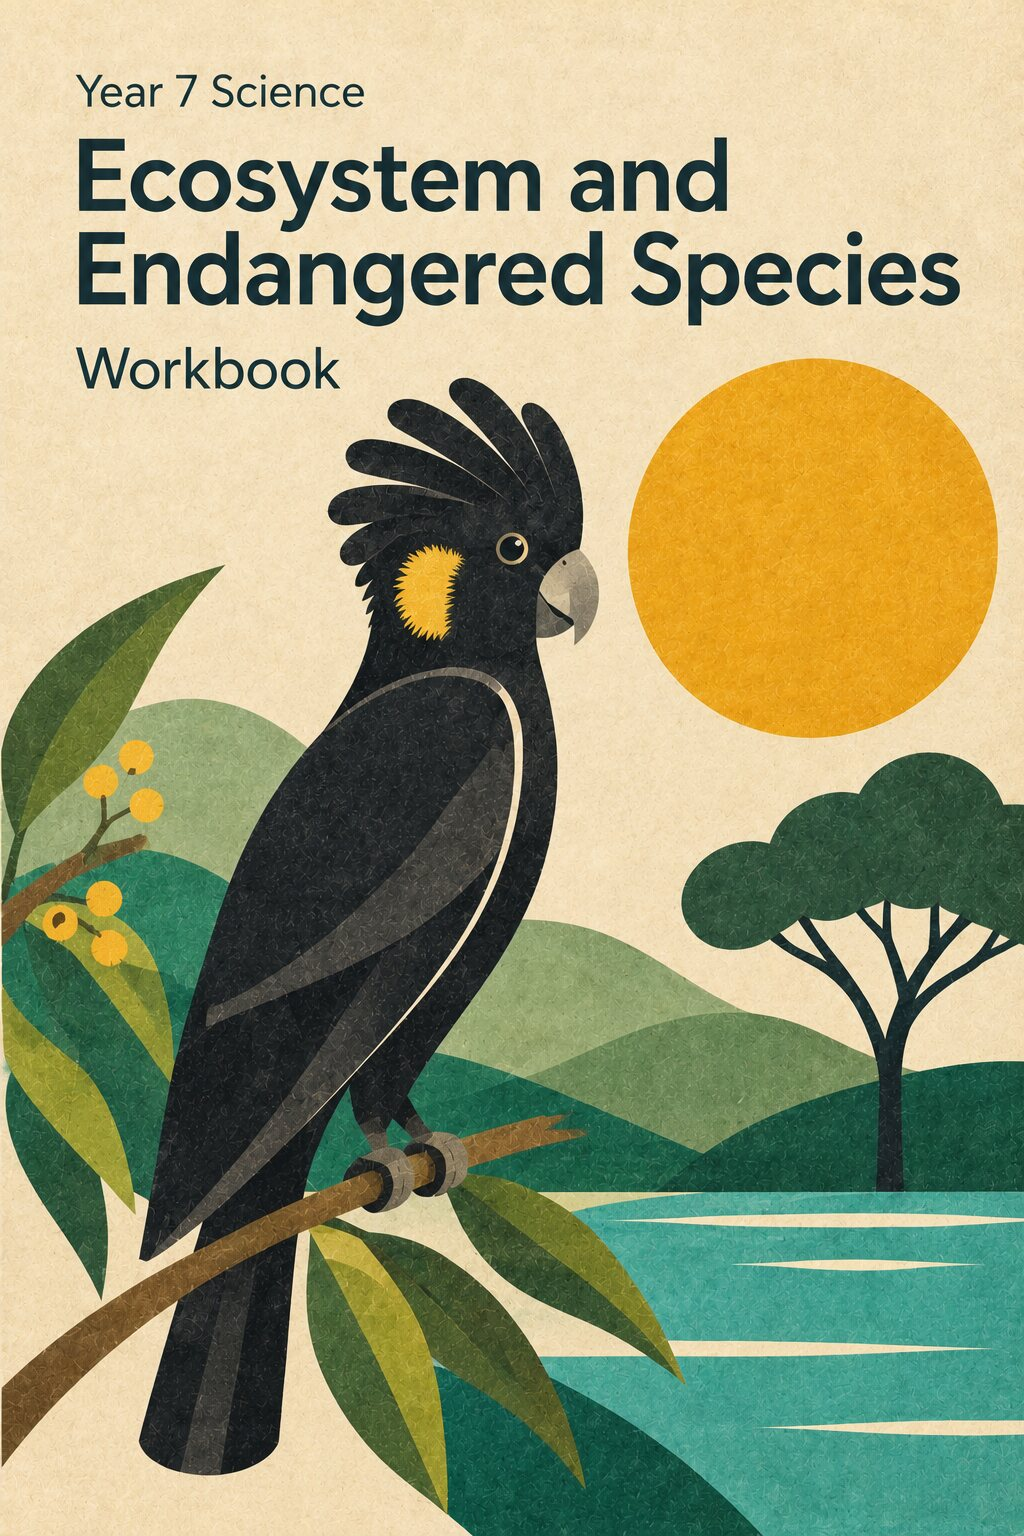
\includegraphics[width=\paperwidth]{../../../covers/ecosystems.jpg}};
  \node[anchor=north east, fill=white, draw=Ink, line width=0.6pt, rounded corners=1.2mm,
        inner xsep=2mm, inner ysep=1.8mm, text width=30mm, font=\headingfont\footnotesize]
    at ([xshift=-4mm, yshift=-4mm]current page.north east)
    {\textbf{Name}\par\vspace{4mm}\hrule\vspace{2mm}\textbf{Class}\par\vspace{4mm}\hrule};
  \node[anchor=south east, fill=white, draw=Ink, line width=0.6pt, rounded corners=1.2mm,
        inner xsep=2.6mm, inner ysep=2mm, font=\headingfont\bfseries, align=right]
    at ([xshift=-4mm, yshift=6mm]current page.south east)
    {Lesson Booklet 2\\[-1pt]{\normalfont\headingfont\scriptsize Lessons 5--8}};
\end{tikzpicture}
\mbox{}
\clearpage

% ---- Inside cover ---------------------------------------------------------
\thispagestyle{plain}
{\headingfont\bfseries\fontsize{22}{26}\selectfont Biodiversity and Ecosystems}\par\vspace{1mm}
{\headingfont\large Lesson Booklet 2 \textbullet\ Lessons 5--8 \textbullet\ Year 7}\par\vspace{1mm}
{\small\itshape VC 2.0: VC2S8U01 \textbullet\ VC2S8U04 \textbullet\ VC2S8I01--I08 \textbullet\ VC2S8H02--H04}\par\vspace{4mm}
\textbf{Teacher}\ \hrulefill\par

\begin{countrybox}{Acknowledgement of Country}
This booklet was created on the unceded Country of the Wurundjeri Woi-wurrung people of the Kulin Nation. We acknowledge Elders past, present and emerging.
\end{countrybox}

\begin{infobox}{How this booklet works}
One section for each lesson. Each opens with its key vocabulary, then:\par\smallskip
\renewcommand{\arraystretch}{1.25}
\begin{tabular}{@{}p{24mm}p{70mm}@{}}
\textbf{Part A} & a reading with comprehension questions \\
\textbf{Part B} & the ideas, worked through \\
\textbf{Part C} & practice on your own \\
\end{tabular}

\smallskip
\begin{tabular}{@{}p{24mm}p{70mm}@{}}
\textbf{I do} \tagicon{\icodots{1}} & your teacher works an example (solid frame) \\
\textbf{We do} \tagicon{\icodots{2}} & you try one together (dashed frame) \\
\textbf{Reading} \tagicon{\icoread} & a passage to read (thin frame) \\
\end{tabular}

\smallskip
Three lesson books. The five labs share a lesson and are in the \textbf{Experiment Booklet}. Finished your lesson work and want to go further? Ask your teacher about \textbf{Advanced Ecosystems}.
\end{infobox}

\clearpage
\markboth{Contents}{Contents}
{\headingfont\bfseries\LARGE Contents}\par\vspace{1mm}\noindent\rule{\linewidth}{0.6pt}\par\vspace{2mm}
\renewcommand{\arraystretch}{1.45}
\begin{tabular}{|C{1.1cm}|L{6.0cm}|C{2.4cm}|}
  \hline\thead{Lesson} & \thead{Title} & \thead{Page} \\ \hline
  1 & \textit{Living or Non-living?} \newline{\footnotesize\itshape + Lab: Is Yeast Alive? (Experiment Booklet)} & Book 1 \\ \hline
  2 & \textit{Classification: Linnaean Levels} & Book 1 \\ \hline
  3 & \textit{Scientific Names and the Six Kingdoms} & Book 1 \\ \hline
  4 & \textit{Dichotomous Keys} \newline{\footnotesize\itshape + Lab: Key the Schoolyard (Experiment Booklet)} & Book 1 \\ \hline
  5 & \hyperlink{lesson.5.1}{Australian Ecosystems and Biodiversity} \newline{\footnotesize\itshape + Lab: Quadrat Survey (Experiment Booklet)} & \hyperlink{lesson.5.1}{p.\ \pageref{sec:5}} \\ \hline
  6 & \hyperlink{lesson.6.1}{Food Webs and Energy Flow} & \hyperlink{lesson.6.1}{p.\ \pageref{sec:6}} \\ \hline
  7 & \hyperlink{lesson.7.1}{Ecosystem Services} & \hyperlink{lesson.7.1}{p.\ \pageref{sec:7}} \\ \hline
  8 & \hyperlink{lesson.8.1}{Adaptations} \newline{\footnotesize\itshape + Lab: Beaks and Food (Experiment Booklet)} & \hyperlink{lesson.8.1}{p.\ \pageref{sec:8}} \\ \hline
  9 & \textit{Introduced Species} \newline{\footnotesize\itshape + Lab: The Rabbit and Fox Model (Experiment Booklet)} & Book 3 \\ \hline
  10 & \textit{Human Impacts on Ecosystems} & Book 3 \\ \hline
  11 & \textit{Conservation and Action} & Book 3 \\ \hline
  --- & \hyperlink{glossary}{Glossary} & \hyperlink{glossary}{\pageref{sec:glossary}} \\ \hline
\end{tabular}
\renewcommand{\arraystretch}{1}
\clearpage
% ══════════════════════════════════════════════════════════════════════════════
%  BIODIVERSITY AND ECOSYSTEMS — A5 LESSON BOOKLET, LESSONS 5–8
% ══════════════════════════════════════════════════════════════════════════════

% ══════════════════════════════════════════════════════════════════════════════
%  LESSON 5 — AUSTRALIAN ECOSYSTEMS AND BIODIVERSITY
% ══════════════════════════════════════════════════════════════════════════════
\setcounter{section}{4}
\sectiondiv{Australian Ecosystems and Biodiversity}{Biotic and abiotic factors \textbullet{} Victorian ecosystems \textbullet{} Three levels of biodiversity}\label{sec:5}
\lessoncodes{VC2S8U04 \textbullet{} VC2S8H02}

\vocabhead
\begin{ctab}
\begin{tabular}{|SW{3.4cm}|W{7.0cm}|}
  \hline\hd & \thead{Word} & \thead{Definition (copy from the slide)} \\ \hline
  & \scaf{\textbf{Ecosystem}\label{voc:ecosystem}} & \scaf{All the living things in an area, together with the non-living surroundings they interact with.} \\ \hline
  & \textbf{Biotic}\label{voc:biotic} & \\ \hline
  & \textbf{Abiotic}\label{voc:abiotic} & \\ \hline
  & \textbf{Habitat}\label{voc:habitat} & \\ \hline
  & \textbf{Biodiversity}\label{voc:biodiversity} & \\ \hline
  & \textbf{Monoculture}\label{voc:monoculture} & \\ \hline
\end{tabular}
\end{ctab}

% ─── PART A ───────────────────────────────────────────────────────────────────
\lessonpart{A}{Reading and comprehension}{Teal}\label{read:5}

\begin{readingbox}{Reading --- From the Alps to the Bay}
Within a day's drive of Melbourne you can stand in snow among twisted snow gums, walk through towering mountain ash forest, cross a flat native grassland, and wade through a salt marsh beside the bay. Each of these is a different \textbf{ecosystem}: a community of living things, together with the non-living surroundings they interact with.

The living parts of an ecosystem are its \textbf{biotic} factors: plants, animals, fungi and bacteria, and even dead leaves and logs, which were once alive. The non-living parts are its \textbf{abiotic} factors: sunlight, temperature, water, soil, wind and rock. The abiotic factors decide which organisms can live there. A snow gum survives months under snow; a saltbush survives salty soil.

The place where an organism lives and finds everything it needs is its \textbf{habitat}. A hollow in an old mountain ash tree is the habitat of a Leadbeater's possum.

The variety of life in an area is its \textbf{biodiversity}. A native grassland can hold dozens of kinds of plants and hundreds of kinds of insects. A wheat paddock is a \textbf{monoculture}: one crop, planted on purpose, with very few other species.
\end{readingbox}

\rcreset
\rcq{What two things make up an ecosystem?}{2.5cm}
\rcq{Give three biotic and three abiotic factors.}{2.5cm}
\rcq{Why is a dead log a biotic factor?}{2cm}
\rcq{How do abiotic factors affect which organisms live in an ecosystem?}{2.5cm}
\rcq{What is a monoculture, and why does it have low biodiversity?}{2.5cm}

% ─── PART B ───────────────────────────────────────────────────────────────────
\lessonpart{B}{Theory and examples}{Blue}\label{theory:5}

\subsection{Biotic and Abiotic Factors}\label{sub:5.1}

\begin{center}
\begin{fitbox}\begin{tikzpicture}[font=\small]
  \draw[Ink, line width=0.8pt, rounded corners=2mm] (-4.9,-2.1) rectangle (-0.9,1.6);
  \draw[Ink, line width=0.8pt, rounded corners=2mm, fill=black!8] (0.9,-2.1) rectangle (4.9,1.6);
  \node[font=\bfseries] at (-2.9,1.2) {Biotic (living)};
  \node[font=\bfseries] at (2.9,1.2) {Abiotic (non-living)};
  \node[align=center, font=\small] at (-2.9,-0.45) {plants and trees\\animals\\fungi and bacteria\\dead leaves and logs};
  \node[align=center, font=\small] at (2.9,-0.45) {sunlight\\temperature\\water and rainfall\\soil, rock and wind};
  \node[draw=Ink, line width=1pt, fill=white, rounded corners=1.2mm, font=\scriptsize\bfseries, align=center, inner sep=3pt] at (0,-0.3) {ECO-\\SYSTEM};
\end{tikzpicture}\end{fitbox}
\figcap{An ecosystem is its biotic and abiotic factors together.}
\end{center}

\begin{workedex}{Biotic or abiotic?}
\textbf{Leaf litter:} biotic --- the leaves were once alive and are made of cells.\\
\textbf{Rainfall:} abiotic --- water was never alive.\\
\textbf{Soil:} both! The sand and clay are abiotic; the bacteria, fungi and worms living in it are biotic.
\end{workedex}

\begin{wedo}{Biotic or abiotic?}
A rock pool at Ricketts Point holds sea water, sea snails, seaweed, sand and a dead crab shell. Sort each into biotic or abiotic.
\answerbox{4cm}
\end{wedo}

\subsection{Three Levels of Biodiversity}\label{sub:5.2}

\begin{skillbox}{Three levels}
\textbf{Genetic diversity:} differences between individuals of the same species. \quad \textbf{Species diversity:} the number and variety of species in an area. \quad \textbf{Ecosystem diversity:} the variety of ecosystem types in a region.
\end{skillbox}

\begin{workedex}{Comparing two areas}
\textbf{Area A:} a native grassland with 12 plant, 8 insect, 5 bird, 2 reptile and 1 mammal species: 28 species.\\
\textbf{Area B:} a wheat paddock with 1 crop and 3 pest insects: 4 species.

\smallskip
Area A has seven times as many species (28 against 4), so its species diversity is far higher. If a drought or a pest hits Area B, there is nothing else to keep the ecosystem going, so it is more likely to collapse.
\end{workedex}

\begin{wedo}{Comparing two areas}
\textbf{Area A:} a wetland with 48 plant, 18 frog, 95 bird and 27 fish species, in four kinds of habitat (marsh, reed beds, open water, river woodland).\\
\textbf{Area B:} irrigated farmland with 6 plant, 5 bird and 2 mammal species, in one habitat.\\
Compare the biodiversity of the two areas. Use numbers from both, and name two levels of biodiversity.
\answerbox{5cm}
\end{wedo}

\begin{countrybox}{First Nations perspectives --- Birrarung, a living ancestor}
For Wurundjeri Woi-wurrung people, the Birrarung (Yarra River) is not just a list of species and abiotic factors: it is a living ancestor, and the health of its plants and animals is the health of Country. Knowing when eels run, when wattle seeds ripen and when swamp wallabies give birth is a detailed knowledge of species, populations and seasons, built over many generations.
\end{countrybox}

% ─── PART C ───────────────────────────────────────────────────────────────────
\lessonpart{C}{Practice}{Amber}\label{prac:5}

\task Sort each item into biotic or abiotic: rainfall, eastern grey kangaroo, leaf litter, rock, soil bacteria, temperature, sunlight, rotting log, wind, mountain ash tree, river water, fungi.
\begin{ctab}
\begin{tabular}{|SW{5.0cm}|W{5.0cm}|}
  \hline\hd & \thead{Biotic (living or once living)} & \thead{Abiotic (never living)} \\ \hline
  & \scaf{Eastern grey kangaroo} & \scaf{Rainfall} \\ \hline
  & & \\ \hline
  & & \\ \hline
  & & \\ \hline
  & & \\ \hline
\end{tabular}
\end{ctab}

\needspace{14\baselineskip}
\task Choose two of these Victorian ecosystems: alpine, wet mountain ash forest, native grassland, coastal salt marsh. Complete the table.
\begin{ctab}
\begin{tabular}{|SW{2.4cm}|W{3.4cm}|W{2.0cm}|W{2.0cm}|}
  \hline\hd & \thead{Ecosystem} & \thead{Abiotic features} & \thead{One plant} & \thead{One animal} \\ \hline
  & \scaf{Alpine} & \scaf{Cold, snow in winter, strong wind} & \scaf{Snow gum} & \scaf{Mountain pygmy possum} \\ \hline
  & & & & \\ \hline
  & & & & \\ \hline
\end{tabular}
\end{ctab}

\needspace{10\baselineskip}
\task Forest X has 50 plant species and forest Y has 30. Explain why forest X is not necessarily more biodiverse, and say what else you would need to know.
\answerbox{5cm}
\newpage


% ══════════════════════════════════════════════════════════════════════════════
%  LESSON 6 — FOOD WEBS AND ENERGY FLOW
% ══════════════════════════════════════════════════════════════════════════════
\setcounter{section}{5}
\sectiondiv{Food Webs and Energy Flow}{Photosynthesis and respiration \textbullet{} Producers, consumers, decomposers \textbullet{} Food chains and webs}\label{sec:6}
\lessoncodes{VC2S8U04 \textbullet{} VC2S8I04 \textbullet{} VC2S8I05}

\vocabhead
\begin{ctab}
\begin{tabular}{|SW{3.4cm}|W{7.0cm}|}
  \hline\hd & \thead{Word} & \thead{Definition (copy from the slide)} \\ \hline
  & \scaf{\textbf{Producer}\label{voc:producer}} & \scaf{An organism that makes its own food from sunlight, such as a plant.} \\ \hline
  & \textbf{Consumer}\label{voc:consumer} & \\ \hline
  & \textbf{Decomposer}\label{voc:decomposer} & \\ \hline
  & \textbf{Food chain}\label{voc:food-chain} & \\ \hline
  & \textbf{Food web}\label{voc:food-web} & \\ \hline
  & \textbf{Apex predator}\label{voc:apex-predator} & \\ \hline
\end{tabular}
\end{ctab}

% ─── PART A ───────────────────────────────────────────────────────────────────
\lessonpart{A}{Reading and comprehension}{Teal}\label{read:6}

\begin{readingbox}{Reading --- Everything Runs on Sunlight}
A wedge-tailed eagle soars over a grassland, hunting. Where does the energy for its flight come from? Follow it back and you always reach the Sun.

Grasses and trees are \textbf{producers}. In their leaves, they use light energy from the Sun to make a sugar called \textbf{glucose} out of carbon dioxide and water. This is photosynthesis, and it is the only way energy enters an ecosystem. The energy is stored in the glucose.

Animals are \textbf{consumers}: they cannot make their own food, so they eat other organisms. A grasshopper eats grass; a magpie eats the grasshopper. When a plant or animal dies, \textbf{decomposers} such as fungi, bacteria and worms break it down and return its nutrients to the soil.

A \textbf{food chain} shows one path that energy takes: grass $\rightarrow$ grasshopper $\rightarrow$ magpie. The arrows point in the direction the energy flows, from the eaten to the eater. Real animals eat more than one thing, so ecologists join many chains into a \textbf{food web}. At the top is the \textbf{apex predator}, like the wedge-tailed eagle, which nothing else hunts.
\end{readingbox}

\rcreset
\rcq{What is the only way energy enters an ecosystem?}{2cm}
\rcq{What is the difference between a producer and a consumer?}{2.5cm}
\rcq{What do decomposers do, and why do ecosystems need them?}{2.5cm}
\rcq{Which way do the arrows point in a food chain?}{2cm}
\rcq{Why do ecologists draw food webs instead of single food chains?}{2.5cm}

% ─── PART B ───────────────────────────────────────────────────────────────────
\lessonpart{B}{Theory and examples}{Blue}\label{theory:6}

\subsection{Photosynthesis and Respiration}\label{sub:6.1}

\begin{skillbox}{Two word equations}
\textbf{Photosynthesis} (producers only, in the leaves, in light):\par
\centerline{carbon dioxide $+$ water $\xrightarrow{\text{light energy}}$ glucose $+$ oxygen}\par\smallskip
\textbf{Respiration} (every living thing, in every cell, day and night):\par
\centerline{glucose $+$ oxygen $\longrightarrow$ carbon dioxide $+$ water $+$ energy}
\end{skillbox}

\begin{center}
\begin{fitbox}\begin{tikzpicture}[font=\small,
  b/.style={draw=Ink, line width=0.9pt, rounded corners=1.5mm, text width=2.9cm, align=center, minimum height=1.2cm},
  ar/.style={-{Stealth[length=5pt]}, line width=0.9pt, Ink}]
  \node[b] (p) at (0,0) {\textbf{Photosynthesis}\\{\scriptsize producers only}};
  \node[b] (r) at (6,0) {\textbf{Respiration}\\{\scriptsize every living thing}};
  \draw[ar] (p.north east) to[bend left=25] node[above, font=\scriptsize]{glucose and oxygen} (r.north west);
  \draw[ar] (r.south west) to[bend left=25] node[below, font=\scriptsize]{carbon dioxide and water} (p.south east);
  \node[font=\scriptsize\bfseries] (s) at (0,1.75) {light energy in};
  \draw[ar, line width=1.4pt] (s) -- (p);
  \node[font=\scriptsize\bfseries, align=center] (h) at (6,-1.9) {energy for life, then lost as heat};
  \draw[ar, line width=1.4pt] (r) -- (h);
\end{tikzpicture}\end{fitbox}
\figcap{Matter goes round and round; energy comes in as light and leaves as heat.}
\end{center}

\begin{workedex}{Three common mistakes}
\textbf{1. Respiration is not breathing.} Breathing moves air in and out of the lungs; respiration is a reaction inside cells. An earthworm respires but has no lungs.\\
\textbf{2. Plants respire too.} In daylight a plant photosynthesises \emph{and} respires; at night it only respires.\\
\textbf{3. Plants do not get their energy from the soil.} Soil gives water and minerals; the energy comes from sunlight.
\end{workedex}

\begin{wedo}{Is the grass respiring?}
At 2\,a.m. there is no light. Is the wallaby grass photosynthesising, respiring, both or neither? Explain.
\answerbox{4cm}
\end{wedo}

\subsection{Food Chains and Webs}\label{sub:6.2}

\begin{center}
\begin{fitbox}\begin{tikzpicture}[font=\scriptsize,
  o/.style={draw=Ink, line width=0.7pt, rounded corners=1mm, fill=white, align=center, inner sep=2.5pt, minimum width=1.9cm, minimum height=0.6cm},
  ar/.style={-{Stealth[length=4pt]}, line width=0.7pt, Ink}]
  \node[o, fill=black!8] (grass) at (-2.4,0) {Wallaby grass};
  \node[o, fill=black!8] (euc) at (2.4,0) {Eucalyptus tree};
  \node[o] (roo) at (-3.6,1.6) {Kangaroo};
  \node[o] (hop) at (-1.2,1.6) {Grasshopper};
  \node[o] (ros) at (1.2,1.6) {Crimson rosella};
  \node[o] (pos) at (3.6,1.6) {Ringtail possum};
  \node[o] (fal) at (0,3.2) {Brown falcon};
  \node[o] (owl) at (3.6,3.2) {Powerful owl};
  \node[o, line width=1.3pt] (eag) at (-2.4,4.6) {Wedge-tailed eagle};
  \draw[ar] (grass) -- (roo); \draw[ar] (grass) -- (hop);
  \draw[ar] (euc) -- (ros); \draw[ar] (euc) -- (pos);
  \draw[ar] (hop) -- (ros);
  \draw[ar] (hop) -- (fal); \draw[ar] (ros) -- (fal);
  \draw[ar] (ros) -- (owl); \draw[ar] (pos) -- (owl);
  \draw[ar] (roo) -- (eag); \draw[ar] (fal) -- (eag);
\end{tikzpicture}\end{fitbox}
\figcap{A Victorian woodland food web. Producers are shaded. Arrows show the energy flow.}
\end{center}

\begin{workedex}{Reading a food web}
\textbf{Food chain from the web:} eucalyptus $\rightarrow$ ringtail possum $\rightarrow$ powerful owl.\\
\textbf{Roles:} eucalyptus is the producer, the possum is a primary consumer (eats a producer), the owl is a secondary consumer (eats a primary consumer).\\
\textbf{The crimson rosella} eats eucalyptus seeds \emph{and} grasshoppers, so it is both a primary and a secondary consumer.
\end{workedex}

\begin{wedo}{Removing a species}
Disease kills 80\% of the grasshoppers. Predict what happens to the brown falcons and to the wallaby grass, and explain using the arrows in the web.
\answerbox{5cm}
\end{wedo}

\begin{countrybox}{First Nations perspectives --- Cultural burning}
Wurundjeri Woi-wurrung people used cultural burning: cool, carefully timed fires that left a patchwork of country at different stages of regrowth. Fresh grass fed kangaroos and wallabies, thick scrub sheltered small animals, and open ground let birds of prey hunt. This patchwork supported complex, stable food webs. When the burning stopped after colonisation, many ecosystems became more uniform, and more fragile.
\end{countrybox}

% ─── PART C ───────────────────────────────────────────────────────────────────
\lessonpart{C}{Practice}{Amber}\label{prac:6}

\task Give the role of each organism and a short reason.
\begin{ctab}
\begin{tabular}{|SW{2.9cm}|W{2.7cm}|W{4.4cm}|}
  \hline\hd & \thead{Organism} & \thead{Role} & \thead{Reason} \\ \hline
  & \scaf{Wallaby grass} & \scaf{Producer} & \scaf{Makes its own food by photosynthesis} \\ \hline
  & Eastern grey kangaroo & & \\ \hline
  & Brown falcon & & \\ \hline
  & Soil bacteria & & \\ \hline
  & Grasshopper & & \\ \hline
  & Wedge-tailed eagle & & \\ \hline
\end{tabular}
\end{ctab}

\needspace{10\baselineskip}
\task Write a food chain of four organisms from this list, with the arrows pointing the right way: grasshopper, wallaby grass, brown falcon, crimson rosella.
\answerbox{3cm}

\needspace{10\baselineskip}
\task A bandicoot eats a beetle larva at midnight and then spends the night digging. Explain how respiration lets it turn the meal into digging.
\answerbox{5cm}

\needspace{10\baselineskip}
\task In a woodland, the wedge-tailed eagle eats kangaroos and brown falcons. Explain why losing an apex predator like the eagle can change a whole ecosystem.
\answerbox{5cm}
\newpage


% ══════════════════════════════════════════════════════════════════════════════
%  LESSON 7 — ECOSYSTEM SERVICES
% ══════════════════════════════════════════════════════════════════════════════
\setcounter{section}{6}
\sectiondiv{Ecosystem Services}{Provisioning, regulating, cultural, supporting \textbullet{} Victorian examples \textbullet{} Losing a service}\label{sec:7}
\lessoncodes{VC2S8U04 \textbullet{} VC2S8H02}

\vocabhead
\begin{ctab}
\begin{tabular}{|SW{3.4cm}|W{7.0cm}|}
  \hline\hd & \thead{Word} & \thead{Definition (copy from the slide)} \\ \hline
  & \scaf{\textbf{Ecosystem service}\label{voc:ecosystem-service}} & \scaf{A benefit that people get from a healthy ecosystem.} \\ \hline
  & \textbf{Provisioning}\label{voc:provisioning} & \\ \hline
  & \textbf{Regulating}\label{voc:regulating} & \\ \hline
  & \textbf{Cultural}\label{voc:cultural} & \\ \hline
  & \textbf{Supporting}\label{voc:supporting} & \\ \hline
  & \textbf{Pollination}\label{voc:pollination} & \\ \hline
\end{tabular}
\end{ctab}

% ─── PART A ───────────────────────────────────────────────────────────────────
\lessonpart{A}{Reading and comprehension}{Teal}\label{read:7}

\begin{readingbox}{Reading --- Melbourne's Free Water Filter}
Most of Melbourne's drinking water falls as rain on mountain ash forests north-east of the city. The forest soaks up the rain, filters it through deep soil and leaf litter, and lets it trickle into the reservoirs so clean that it needs very little treatment. No machine does this. A healthy forest does it for free.

The benefits people get from healthy ecosystems are called \textbf{ecosystem services}. Scientists sort them into four groups. \textbf{Provisioning} services are the things we take: food, fresh water, timber and medicines. \textbf{Regulating} services keep conditions steady: forests store carbon, wetlands slow floods and clean water, and insects carry out \textbf{pollination}, moving pollen between flowers so that fruit and seeds form. \textbf{Cultural} services feed the mind and spirit: bushwalks, beaches, tourism, and places of deep cultural meaning. \textbf{Supporting} services keep everything else running: making soil, recycling nutrients and providing habitat.

Most ecosystem services go unnoticed --- until they are lost.
\end{readingbox}

\rcreset
\rcq{How does the mountain ash forest help Melbourne's water supply?}{2.5cm}
\rcq{Name the four groups of ecosystem services, with one example of each.}{3cm}
\rcq{What is pollination, and why do farmers need it?}{2.5cm}
\rcq{Why do people often not notice ecosystem services?}{2cm}

% ─── PART B ───────────────────────────────────────────────────────────────────
\lessonpart{B}{Theory and examples}{Blue}\label{theory:7}

\subsection{Four Kinds of Service}\label{sub:7.1}

\begin{ctab}
\begin{tabular}{|L{2.2cm}|L{3.8cm}|L{4.0cm}|}
  \hline\thead{Service} & \thead{What it includes} & \thead{Victorian example} \\ \hline
  Provisioning & Food, water, timber, medicines & Drinking water from mountain ash catchments \\ \hline
  Regulating & Carbon storage, flood control, pollination, cleaning water & Wetlands filtering farm runoff \\ \hline
  Cultural & Recreation, tourism, spiritual connection & Great Ocean Road; the Birrarung's cultural meaning \\ \hline
  Supporting & Making soil, recycling nutrients, habitat & Fungi and bacteria breaking down leaf litter \\ \hline
\end{tabular}
\end{ctab}

\begin{workedex}{Tracing the loss of a service}
Native bee numbers fall by half.

\smallskip
\textbf{Regulating:} pollination of crops and native plants falls.\\
\textbf{Provisioning:} smaller harvests of apples, almonds and blueberries; food costs more.\\
\textbf{Supporting:} native plants make fewer seeds, so less habitat for insects, birds and mammals.\\
\textbf{Conclusion:} losing one service causes losses in the others, because they are all linked.
\end{workedex}

\begin{wedo}{Tracing the loss of a service}
A coastal mangrove forest is cleared for a marina. Mangroves shelter young fish and absorb the energy of storm waves. Trace the effects on two kinds of ecosystem service.
\answerbox{5cm}
\end{wedo}

\begin{countrybox}{First Nations perspectives --- Caring for Country}
Caring for Country means looking after all of Country's services at once, as a relationship of responsibility, not as a set of benefits. Rules against over-harvesting and seasonal management kept food and water plentiful for tens of thousands of years; cultural burning kept land healthy and controlled fire. Research now finds that Country managed by First Nations people often has higher biodiversity than similar land managed in other ways.
\end{countrybox}

% ─── PART C ───────────────────────────────────────────────────────────────────
\lessonpart{C}{Practice}{Amber}\label{prac:7}

\task Name the best-fit service for each, with a reason.
\begin{ctab}
\begin{tabular}{|SW{4.0cm}|W{2.4cm}|W{3.6cm}|}
  \hline\hd & \thead{Example} & \thead{Service} & \thead{Reason} \\ \hline
  & \scaf{Native bees pollinating crops} & \scaf{Regulating} & \scaf{Keeps a natural process working} \\ \hline
  & Birrarung supplying fresh water & & \\ \hline
  & Mangroves absorbing wave energy & & \\ \hline
  & Soil bacteria breaking down dead leaves & & \\ \hline
  & Snowy Mountains drawing ski tourists & & \\ \hline
  & Wetlands filtering farm runoff & & \\ \hline
\end{tabular}
\end{ctab}

\needspace{14\baselineskip}
\task The Birrarung (Yarra River) gives Melbourne many services. For each group, name one service and what would be lost if the river were badly polluted.
\begin{ctab}
\begin{tabular}{|SW{2.3cm}|W{3.6cm}|W{4.1cm}|}
  \hline\hd & \thead{Service} & \thead{What the Birrarung gives} & \thead{Lost if polluted} \\ \hline
  & \scaf{Provisioning} & \scaf{Fresh water} & \scaf{Safe water for drinking and farms} \\ \hline
  & Regulating & & \\ \hline
  & Cultural & & \\ \hline
  & Supporting & & \\ \hline
\end{tabular}
\end{ctab}

\needspace{10\baselineskip}
\task Explain why losing biodiversity leads to losing ecosystem services.
\answerbox{5cm}
\newpage


% ══════════════════════════════════════════════════════════════════════════════
%  LESSON 8 — ADAPTATIONS
% ══════════════════════════════════════════════════════════════════════════════
\setcounter{section}{7}
\sectiondiv{Adaptations}{Structural, behavioural, physiological \textbullet{} Victorian species \textbullet{} Suited to a place}\label{sec:8}
\lessoncodes{VC2S8U04 \textbullet{} VC2S8H02}

\vocabhead
\begin{ctab}
\begin{tabular}{|SW{3.4cm}|W{7.0cm}|}
  \hline\hd & \thead{Word} & \thead{Definition (copy from the slide)} \\ \hline
  & \scaf{\textbf{Adaptation}\label{voc:adaptation}} & \scaf{An inherited feature that helps an organism survive and reproduce where it lives.} \\ \hline
  & \textbf{Structural}\label{voc:structural} & \\ \hline
  & \textbf{Behavioural}\label{voc:behavioural} & \\ \hline
  & \textbf{Physiological}\label{voc:physiological} & \\ \hline
  & \textbf{Torpor}\label{voc:torpor} & \\ \hline
  & \textbf{Nocturnal}\label{voc:nocturnal} & \\ \hline
\end{tabular}
\end{ctab}

% ─── PART A ───────────────────────────────────────────────────────────────────
\lessonpart{A}{Reading and comprehension}{Teal}\label{read:8}

\begin{readingbox}{Reading --- The Echidna's Toolkit}
The short-beaked echidna lives everywhere from the Victorian Alps to the desert. It survives because of its \textbf{adaptations}: inherited features that help it survive and reproduce where it lives.

Some adaptations are body parts. These are \textbf{structural} adaptations. The echidna's spines are hairs made hard and sharp; when an eagle or a quoll attacks, the echidna digs in or curls up so only spines show. Its tongue, up to 18\,cm long and sticky, reaches deep into ant nests.

Some are things an animal does: \textbf{behavioural} adaptations. Echidnas shelter in logs and burrows in cold weather, and in hot areas they are \textbf{nocturnal}, active at night when it is cooler.

Others happen inside the body: \textbf{physiological} adaptations. In winter, when ants are scarce, an echidna goes into \textbf{torpor}: its body temperature, heart rate and breathing drop, saving energy until food returns.

An adaptation is not something an animal decides to grow. It is inherited, passed from parents to young over many generations.
\end{readingbox}

\rcreset
\rcq{What is an adaptation?}{2cm}
\rcq{Give one structural adaptation of the echidna and how it helps.}{2.5cm}
\rcq{Give one behavioural adaptation of the echidna and how it helps.}{2.5cm}
\rcq{What happens to an echidna during torpor, and why is it useful in winter?}{2.5cm}
\rcq{Why can an animal not simply choose to grow an adaptation?}{2.5cm}

% ─── PART B ───────────────────────────────────────────────────────────────────
\lessonpart{B}{Theory and examples}{Blue}\label{theory:8}

\subsection{Three Types of Adaptation}\label{sub:8.1}

\begin{center}
\begin{fitbox}\begin{tikzpicture}[font=\small,
  t/.style={draw=Ink, rounded corners=1.5mm, text width=2.9cm, align=center, minimum height=2.2cm, inner sep=3pt}]
  \node[t, line width=0.8pt] at (0,0) {\textbf{Structural}\\[2pt]{\scriptsize body parts:\\fur, spines, webbed feet, camouflage}};
  \node[t, line width=0.8pt, dashed] at (3.4,0) {\textbf{Behavioural}\\[2pt]{\scriptsize what it does:\\migration, sheltering, being nocturnal}};
  \node[t, line width=0.8pt, double, double distance=1.2pt] at (6.8,0) {\textbf{Physiological}\\[2pt]{\scriptsize inside the body:\\torpor, concentrated urine, venom}};
\end{tikzpicture}\end{fitbox}
\figcap{Three types of adaptation.}
\end{center}

\begin{workedex}{Classifying adaptations}
\textbf{Kangaroo's large hind legs:} structural --- a body part; hopping uses little energy over long distances to find food and water.\\
\textbf{Kangaroo licking its forearms in heat:} behavioural --- an action; evaporating saliva cools the blood.\\
\textbf{Kangaroo making very concentrated urine:} physiological --- inside the body; it saves water in dry country.
\end{workedex}

\begin{wedo}{Classifying adaptations}
The tawny frogmouth has grey, streaky feathers like tree bark, and sits very still on a branch during the day with its beak pointed up. Name two adaptations, classify each, and explain how they work together.
\answerbox{5cm}
\end{wedo}

\subsection{Suited to One Place}\label{sub:8.2}

\begin{workedex}{The mountain pygmy possum}
The mountain pygmy possum lives only above 1400\,m in the Victorian Alps. It hibernates under the snow for up to seven months (physiological), and it stores seeds for winter (behavioural).

\smallskip
In a Melbourne garden these would not help: there is no snow blanket to keep it at a steady temperature, so hibernating would waste energy, and its main food, the bogong moth, does not gather there.
\end{workedex}

\begin{wedo}{Suited to one place}
A little penguin has stiff, flipper-like wings and a thick layer of fat. Explain why these suit the sea, and why they would be a poor fit in a dry inland woodland.
\answerbox{5cm}
\end{wedo}

\begin{countrybox}{First Nations perspectives --- Knowing animals' habits}
Kulin Nation peoples travelled to the high country each summer for the feast of bogong moths, which shelter in alpine rock crevices to escape the lowland heat. Knowing exactly when and where the moths gathered, and when echidnas went into torpor, came from tens of thousands of years of careful observation of animal adaptations and behaviour. It is ecological science in its own right.
\end{countrybox}

% ─── PART C ───────────────────────────────────────────────────────────────────
\lessonpart{C}{Practice}{Amber}\label{prac:8}

\task Classify each adaptation as structural (S), behavioural (B) or physiological (P), and explain how it helps.
\begin{ctab}
\begin{tabular}{|SW{3.5cm}|Z{1.0cm}|W{5.5cm}|}
  \hline\hd & \thead{Adaptation} & \thead{S/B/P} & \thead{How it helps} \\ \hline
  & \scaf{Kangaroo: large hind legs} & \scaf{S} & \scaf{Hops long distances using little energy} \\ \hline
  & Tawny frogmouth: bark-like feathers & & \\ \hline
  & Echidna: body cools in winter & & \\ \hline
  & Platypus: bill senses electric signals & & \\ \hline
  & Ringtail possum: active at night & & \\ \hline
  & Wombat: pouch opens backwards & & \\ \hline
\end{tabular}
\end{ctab}

\needspace{14\baselineskip}
\task Describe one adaptation of the platypus of each type.
\begin{ctab}
\begin{tabular}{|SW{2.3cm}|W{3.2cm}|W{4.5cm}|}
  \hline\hd & \thead{Type} & \thead{Adaptation} & \thead{How it helps survival} \\ \hline
  & \scaf{Structural} & \scaf{Webbed front feet} & \scaf{Paddles through water to catch food} \\ \hline
  & Behavioural & & \\ \hline
  & Physiological & & \\ \hline
\end{tabular}
\end{ctab}

\needspace{10\baselineskip}
\task Explain why an adaptation that helps an animal in one ecosystem can be useless in another. Use an example.
\answerbox{5cm}
\newpage

\clearpage\markboth{Glossary}{Glossary}\hypertarget{glossary}{}\pdfbookmark[1]{Glossary}{glossarybm}
{\headingfont\bfseries\LARGE Glossary}\label{sec:glossary}\par\vspace{1mm}\noindent\rule{\linewidth}{0.6pt}\par
{\small Every key word in this booklet and the page it is introduced on.}\par\smallskip
\renewcommand{\arraystretch}{1.3}
\begin{longtable}{|>{\RaggedRight}p{34mm}|p{9mm}|p{\dimexpr\linewidth-43mm-6\tabcolsep-4\arrayrulewidth-1pt\relax}|}
\hline \rule{0pt}{4mm}\headingfont\bfseries Word & \headingfont\bfseries Page & \headingfont\bfseries In my own words \\ \hline \endhead
  Abiotic & \pageref{voc:abiotic} & \\ \hline
  Adaptation & \pageref{voc:adaptation} & \\ \hline
  Apex predator & \pageref{voc:apex-predator} & \\ \hline
  Behavioural & \pageref{voc:behavioural} & \\ \hline
  Biodiversity & \pageref{voc:biodiversity} & \\ \hline
  Biotic & \pageref{voc:biotic} & \\ \hline
  Consumer & \pageref{voc:consumer} & \\ \hline
  Cultural & \pageref{voc:cultural} & \\ \hline
  Decomposer & \pageref{voc:decomposer} & \\ \hline
  Ecosystem & \pageref{voc:ecosystem} & \\ \hline
  Ecosystem service & \pageref{voc:ecosystem-service} & \\ \hline
  Food chain & \pageref{voc:food-chain} & \\ \hline
  Food web & \pageref{voc:food-web} & \\ \hline
  Habitat & \pageref{voc:habitat} & \\ \hline
  Monoculture & \pageref{voc:monoculture} & \\ \hline
  Nocturnal & \pageref{voc:nocturnal} & \\ \hline
  Physiological & \pageref{voc:physiological} & \\ \hline
  Pollination & \pageref{voc:pollination} & \\ \hline
  Producer & \pageref{voc:producer} & \\ \hline
  Provisioning & \pageref{voc:provisioning} & \\ \hline
  Regulating & \pageref{voc:regulating} & \\ \hline
  Structural & \pageref{voc:structural} & \\ \hline
  Supporting & \pageref{voc:supporting} & \\ \hline
  Torpor & \pageref{voc:torpor} & \\ \hline
\end{longtable}
\padtofour
\end{document}
